%%%%%%%%%%%%%%%%%%%%%%%%%%%%%%%%%%%%%%%%%

%----------------------------------------------------------------------------------------
%	PACKAGES AND OTHER DOCUMENT CONFIGURATIONS
%----------------------------------------------------------------------------------------

\documentclass[a4paper,10pt]{article}

\usepackage[utf8]{inputenc} % Required for inputting international characters
\usepackage[T1]{fontenc} % Output font encoding for international characters
% !TEX encoding = UTF-8 Unicode
%\usepackage[utf8]{inputenc}
\usepackage{pdfpages}
\usepackage{mathtools}
\usepackage{amsmath}
\usepackage{fullpage}
\usepackage{bm}
\usepackage{float}
\usepackage{gensymb}
\graphicspath{./dir/} 
\usepackage{mathpazo} % Palatino font


\begin{document}

%----------------------------------------------------------------------------------------
%	TITLE PAGE
%----------------------------------------------------------------------------------------

\begin{titlepage} % Suppresses displaying the page number on the title page and the subsequent page counts as page 1
	\newcommand{\HRule}{\rule{\linewidth}{0.5mm}} % Defines a new command for horizontal lines, change thickness here
	
	\center % Centre everything on the page
	
	%------------------------------------------------
	%	Headings
	%------------------------------------------------

	
	\textsc{\LARGE University of Oslo}\\[1.5cm] % Main heading such as the name of your university/college
	
	\textsc{\Large Control of Mobile Robots}\\[0.5cm] % Major heading such as course name
	
	\textsc{\large UNIK4490}\\[0.5cm] % Minor heading such as course title
	
	%------------------------------------------------
	%	Title
	%------------------------------------------------
	
	\HRule\\[0.4cm]
	
	{\huge\bfseries Odometry and Posture Regulation for a 4 by 4 mobile robot}\\[0.4cm] % Title of your document
	\HRule\\[0.8cm]
	{\large{Autumn 2017}} % Date, change the \today to a set date if you want to be precise	
	\vspace{1cm}
	%------------------------------------------------
	%	Author(s)
	%------------------------------------------------
	
	\begin{minipage}{0.4\textwidth}
		\begin{flushleft}
			\large
			\textit{Authors}\\
			Eirik \textsc{Kvalheim}, Daniel \textsc{Sander Isaksen} and Torgrim \textsc{R. Næss}
		\end{flushleft}
	\end{minipage}
	~
	\begin{minipage}{0.4\textwidth}
		\begin{flushright}
			\large
			\textit{Supervisors}\\
			Dr. Kim \textsc{Mathiassen} and Magnus \textsc{Baksaas}
		\end{flushright}
	\end{minipage}
	
	% If you don't want a supervisor, uncomment the two lines below and comment the code above
	%{\large\textit{Author}}\\
	%John \textsc{Smith} % Your name
	
	%------------------------------------------------
	%	Date
	%------------------------------------------------
	
	\vfill\vfill\vfill\vfill\vfill\vfill\vfill\vfill\vfill\vfill\vfill\vfil\vfill\vfill\vfill\vfill\vfill\vfill\vfill\vfill\vfill\vfill\vfill\vfill\vfill\vfill\vfill\vfill%  go wild
	
	
	%------------------------------------------------
	%	Logo
	%------------------------------------------------
	
	%\vfill\vfill
	%\includegraphics[width=0.2\textwidth]{placeholder.jpg}\\[1cm] % Include a department/university logo - this will require the graphicx package
	\begin{figure}[H]
	\raggedright
	 
\includegraphics[width=0.15\textwidth]{uiologo.png}
	\end{figure}
	 
	%----------------------------------------------------------------------------------------
	
	\vfill % Push the date up 1/4 of the remaining page
	
\end{titlepage}

%----------------------------------------------------------------------------------------


\renewcommand{\labelenumi}{\alph{enumi})}


	\begin{figure}[H]
	\centering
	 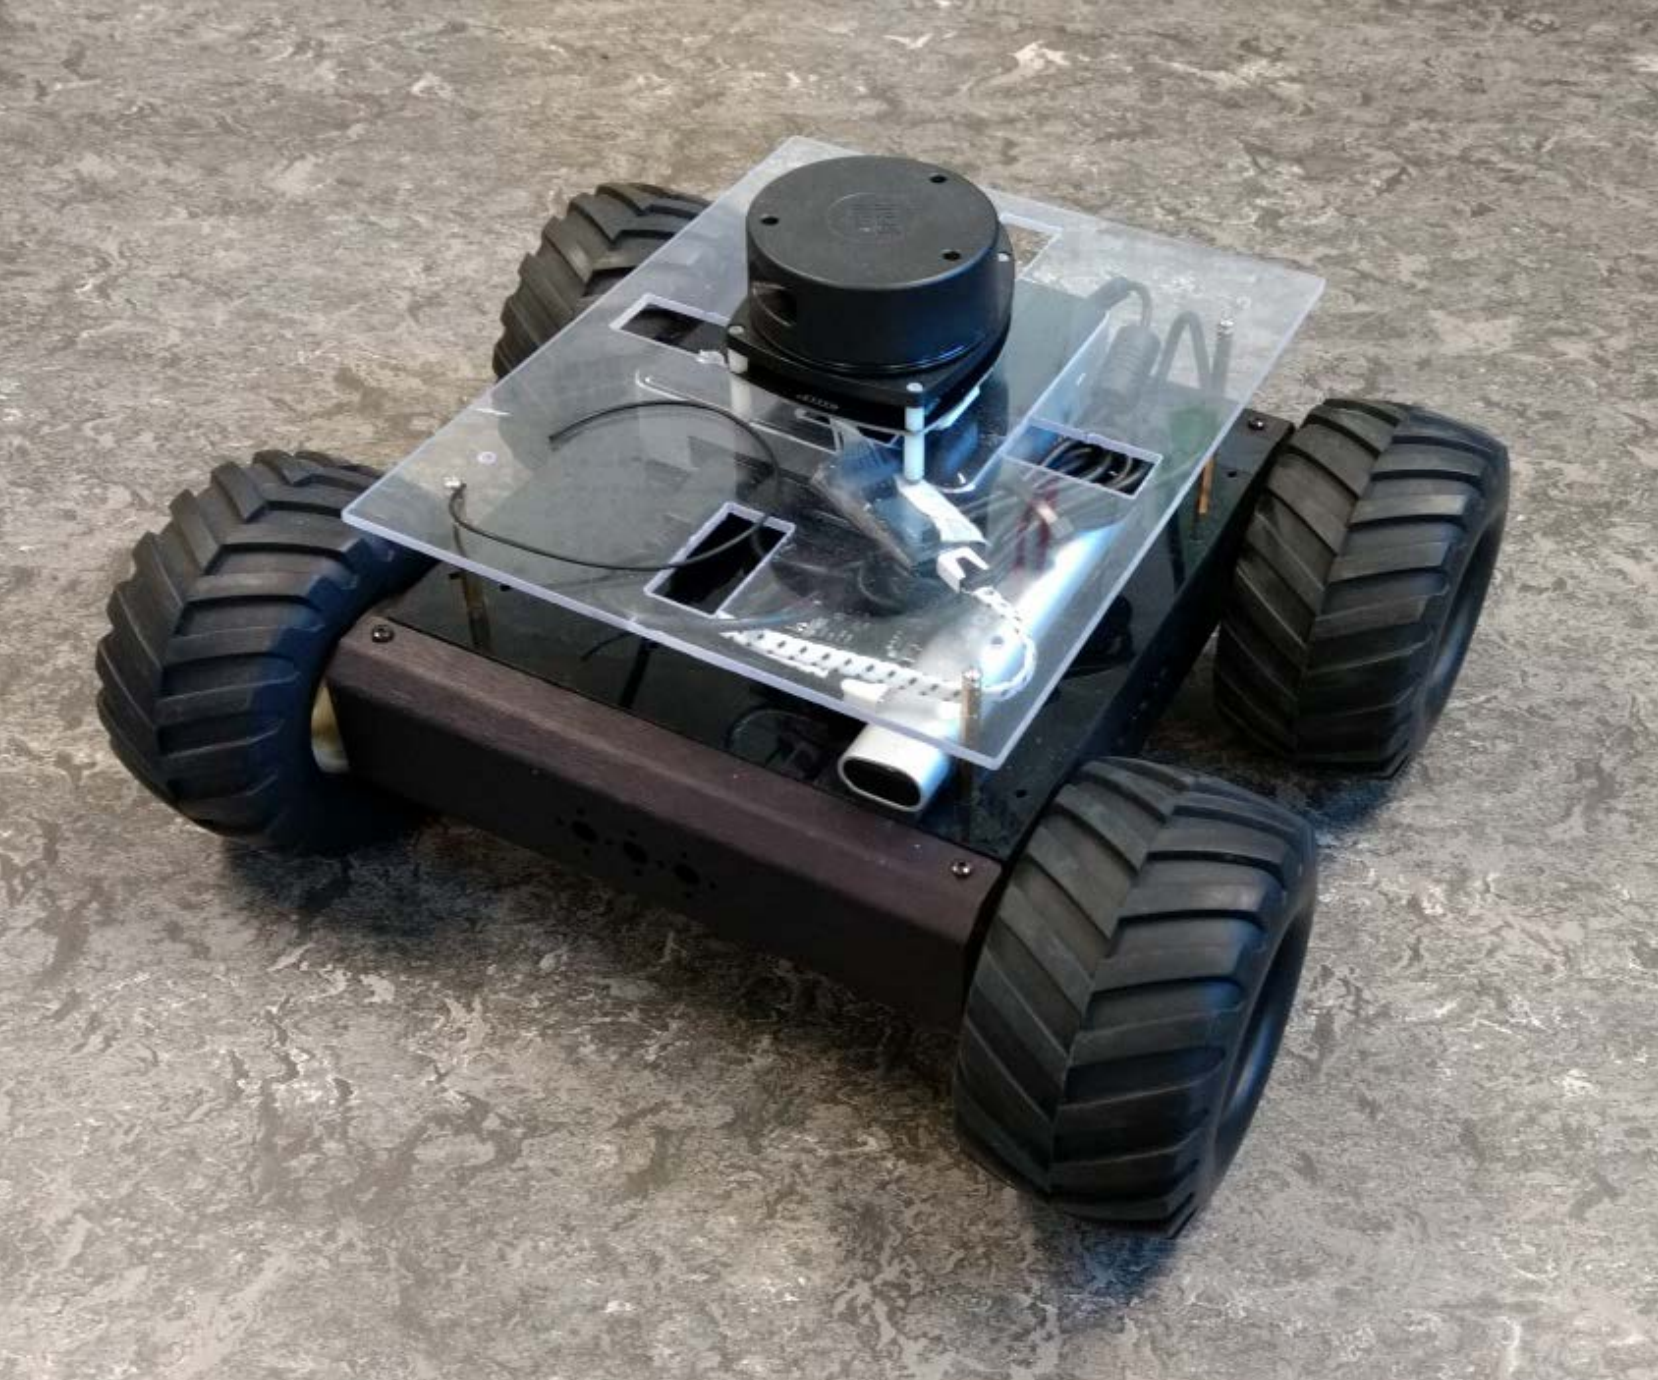
\includegraphics[width=0.5\textwidth]{rover_pic.png}
	%\caption{Rover}	
 	%\label{fig:1}
	\end{figure}

\section{Introduction}
The main goal of this project was to implement motor control, posture regulation and odometric localization in order to get the robot to move to a desired pose. We were working on an existing software stack running ROS (Robot Operating System), so getting to know the previous software aswell as ROS as a system, was also a goal in this project.\\
A significant portion of the project time was spent on reverse engineering the robot to better understand the system in order to implement our own solutions. In the end we had also spent a lot of time on tuning the regulator parameters, aswell as compensating for odometric faulties. Most of the work was done in collaboration with another group that were working on an identical robot with the same software stack. \\

\section{The System}
Figure 1 illustrates our implementation of the system with control loop. It consists of posture regulaton, motor controller, kinematic model, and odometry. Here we are setting a desired pose, and the posture regulator tries to drive the error towards 0.

	\begin{figure}[H]
	\centering
	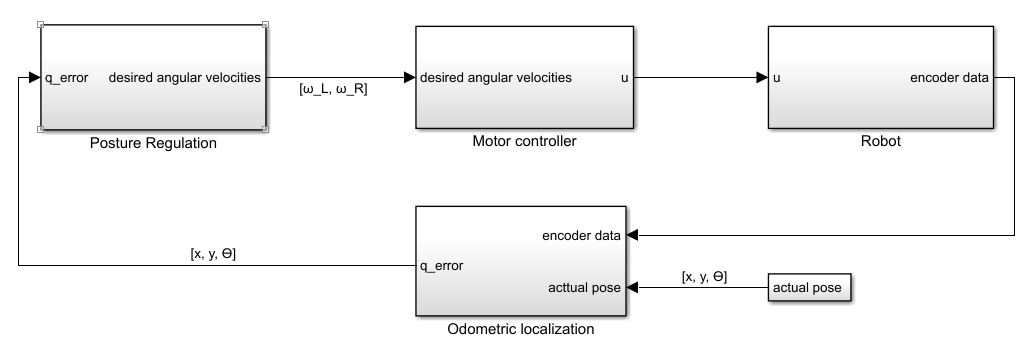
\includegraphics[width=0.9\textwidth]{blokkskjema.JPG}
	\caption{System with Control loop}	
 	\label{fig:2}
	\end{figure}

\subsection{Kinematic Model}
We used the kinematic model of a unicycle derived in chapter 11.2.1 in "Robotics - Modelling, Planning and Control" by B. Siciliano et.al. Here $v$ is the driving velocity and $\omega$ is the steering velocity.

\begin{equation}
	\begin{bmatrix}
	\dot{x}\\ 
	\dot{y}\\
	\dot{\theta}\\  
	\end{bmatrix}
	=
	\begin{bmatrix}
	cos\theta\\ 
	sin\theta\\
	0\\  
	\end{bmatrix}v
	+
	\begin{bmatrix}
	0\\ 
	0\\
	1\\  
	\end{bmatrix}\omega
\end{equation}


\subsection{Motor Control}
	The implementation of motor control for each wheel was already available in the software stack. We started our project by reverse engineering the code in order to get the motor driver to work.
This motordriver/controller had an internal pid regulator, and uses encoder data to calculate wheel velocities. 
	As we were not familiar with the system, and since there were no documentation or comments in the code, we faced challenges on elementary problems as; communication with the robot, running the motordriver and deducing the reason behind the constants in the controller.
In the end it turned out that there was an usb port which needed to be taken in and out every time the motordriver runs the first time. This was the usb connecting the teensy that reads the encoders. There are still unknown constants in this code that has an effect on the published velocity, so we cannot know if this motordriver is publishing correct speeds or not. We ended up assuming that it was correct and moved on to derive the odometry and posture regulator.
	

\subsection{Odometric Localization}

		
		\begin{equation}
		x_{k+1}=x_k+\frac{v_k}{\omega_k}(sin\theta_{k+1}-sin\theta_k)
		\end{equation}
		\begin{equation}
		y_{k+1}=y_k+\frac{v_k}{\omega_k}(cos\theta_{k+1}-cos\theta_k)
		\end{equation}
		\begin{equation}
		\theta_{k+1}=\theta_k+\omega_kT_s
		\end{equation}

		We do this by subscribing to the topic \textit{/est\_vel} which is published from the motordriver.

		
\subsection{Posture Regulation}

	
		We have implemented posture control from chapter 11.6.2 in  "Robotics - Modelling, Planning and Control" by B. Siciliano et.al. 
		In general the posture regulation controller takes in the configuration vector $q = [x, y, \theta]^{T}$ (Cartesian position and vehicle orientation), 
		and outputs v and $\omega$.
		It is assumed that the desired variables are $q_{d} = [0, 0, 0]^{T}$ and the error from $q_{d}$ is represented by
		\begin{equation}
			\rho = \sqrt{x^{2} + y^{2}} 
		\end{equation}
		\begin{equation}
			\gamma = Atan2(y, x) - \theta + \pi
		\end{equation}
		\begin{equation}
			\delta = \gamma + \theta
		\end{equation}
		where $\rho = ||\vec{e_{p}}||$ is the distance between current point $(x, y)$ and desired point $(0, 0)$, 
		$\gamma$ is the angle between $\vec{e_{p}}$	and the sagittal axis of the vehicle and $\delta$ is the axis between $\vec{e_{p}}$ and the x-axis.	
		v and $\omega$ are found by:
		\begin{equation}
			v = k_{1}\rho cos(\gamma)
		\end{equation}		
		\begin{equation}
			\omega = k_{2}\gamma + k_{1}\frac{sin(\gamma)cos(\gamma)}{\gamma}(\gamma + k_{3}\delta)
		\end{equation}
		
		In our implementation of the controller we get $\vec{q}$ from the odometric module and output $\omega_{R}$ and $\omega_{L}$ to the motor controller. 
		This is done by publishing the angular velocities to the topic \textit{/cmd\_vel}, which the motordriver subscribes on in order to control the velocities.
		Equations for $\omega_{R}$ and $\omega_{L}$ expressed by error variables $\rho$, $\gamma$ and $\delta$, can be found
		by setting equation (3) and (4) equal to equation (1) and (2) respectively, 
		\begin{equation}
			v = \frac{r(\omega_{R} + \omega_{L})}{2}
		\end{equation}
		\begin{equation}
			\omega = \frac{r(\omega_{R} - \omega_{L})}{d}
		\end{equation}
		and then solving for $\omega_{R}$ and $\omega_{L}$. This yields:		
		\begin{equation}
			\omega_{R} = \frac{2k_{1}\rho cos(\gamma)}{2r} + \frac{k_{2}d\gamma}{2r} + \frac{k_{1}dsin(\gamma)cos(\gamma)(\gamma + k_{3}\delta)}{2r\gamma}
		\end{equation}
		\begin{equation}
			\omega_{L} = \frac{2k_{1}\rho cos(\gamma)}{2r} - \frac{k_{2}d\gamma}{2r} - \frac{k_{1}dsin(\gamma)cos(\gamma)(\gamma + k_{3}\delta)}{2r\gamma}
		\end{equation}

		Where $d$ is the distance between the outer gripping point of the wheels (almost width of the rover), and $k_{1}$, $k_{2}$ and $k_{3}$ are the controller gains.
		It is woth noting that in equation (6) we are using atan2, which is a function that is undefined in $x=y=0$, therefore $\gamma$ and $\delta$ is also undefined for $x=y=0$.
		To avoid this problem we designed the controller to accept the position and orientation if each element of $q$ had less then 0.05 error. At first, while trying to adjust controller gains 
		we also tried to modify the controller further than the litterature did, to account for the weaknesses. We had no luck with this and ended up with coding exactly the controller
		derived from the litterature, which we then later understood already are proven asymptotically stable given the lyapunov candidate function

\section{Testing and Results}

		When we got all the nodes together our system looked like this;

		\begin{figure}[H]
		\centering
		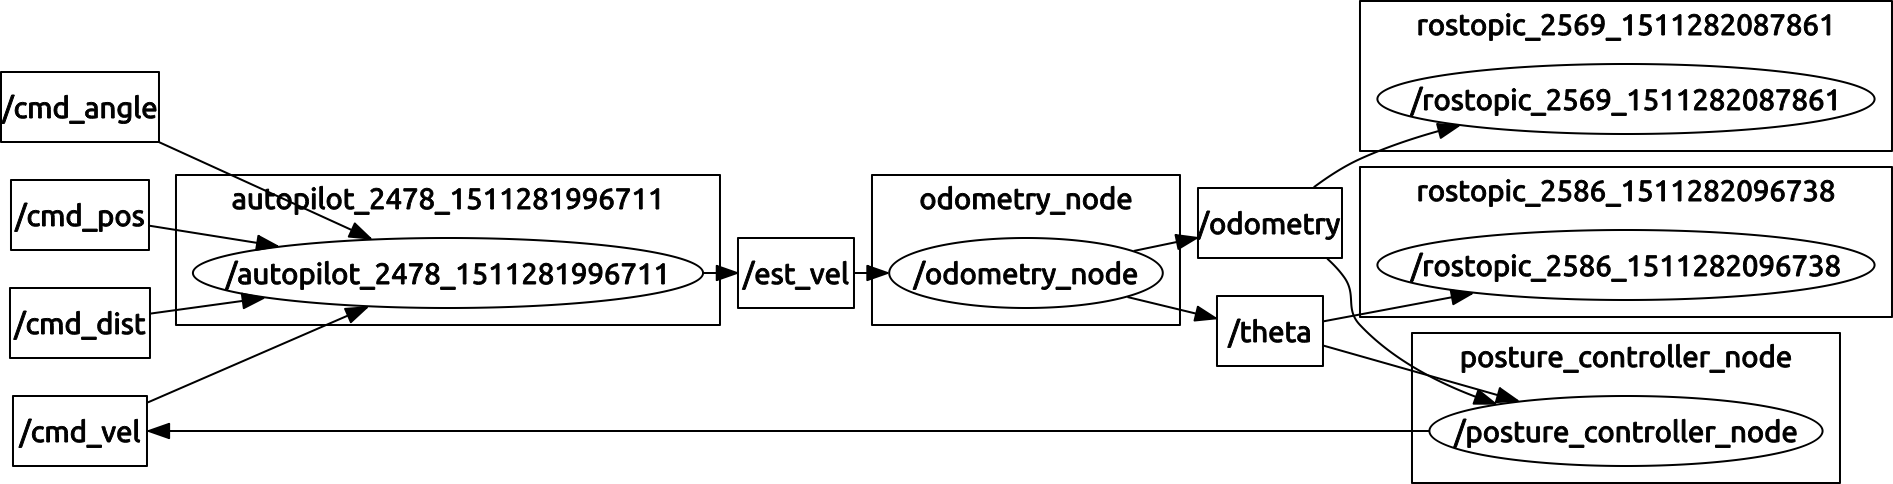
\includegraphics[width=0.9\textwidth]{rover2_rqt_graph.png}
		%\caption{code}	
 		%\label{fig:3}
		\end{figure}

		And as expected one can see assemblance to figure 1. Here you can see the motordriver labled as the node \textit{/autopilot}. \\


		In order to compensate for drift in the odometry, and wrong/estimated velocities (assumption) from the motordriver, we added a factor on the velocity like this;
		\begin{figure}[H]
		\centering
		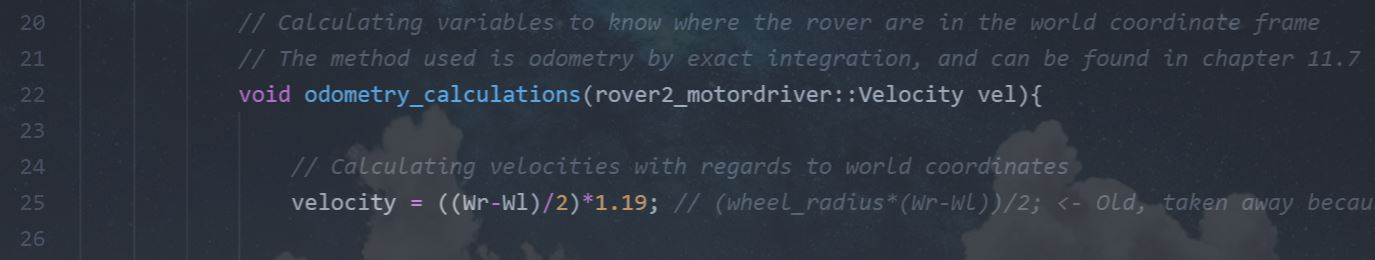
\includegraphics[width=0.9\textwidth]{snippet_adjustment_factor.JPG}
		%\caption{code}	
 		%\label{fig:3}
		\end{figure}
		It turned out 1.19 times the velocity gave us a pretty good result (cm tolerances), which confirmed our suspicion regarding the unknown constants in the motordriver.\\

		We started by implementing the reccomended gains (from the litterature) K1= 1 K2 = 2.5 K3=3, but that did not give us a good regulator.
		Reflecting on the equations (8-13) and discussing which gains we needed to increase with regards to how the robot behaved, we came up with 2 2.3 1.3 wich was a pretty good regulator, with some accuracy problem. Increasing to 2 4 1.3 gave us a more accurate regulator, which also was quicker.

		\begin{figure}[H]
		\centering
		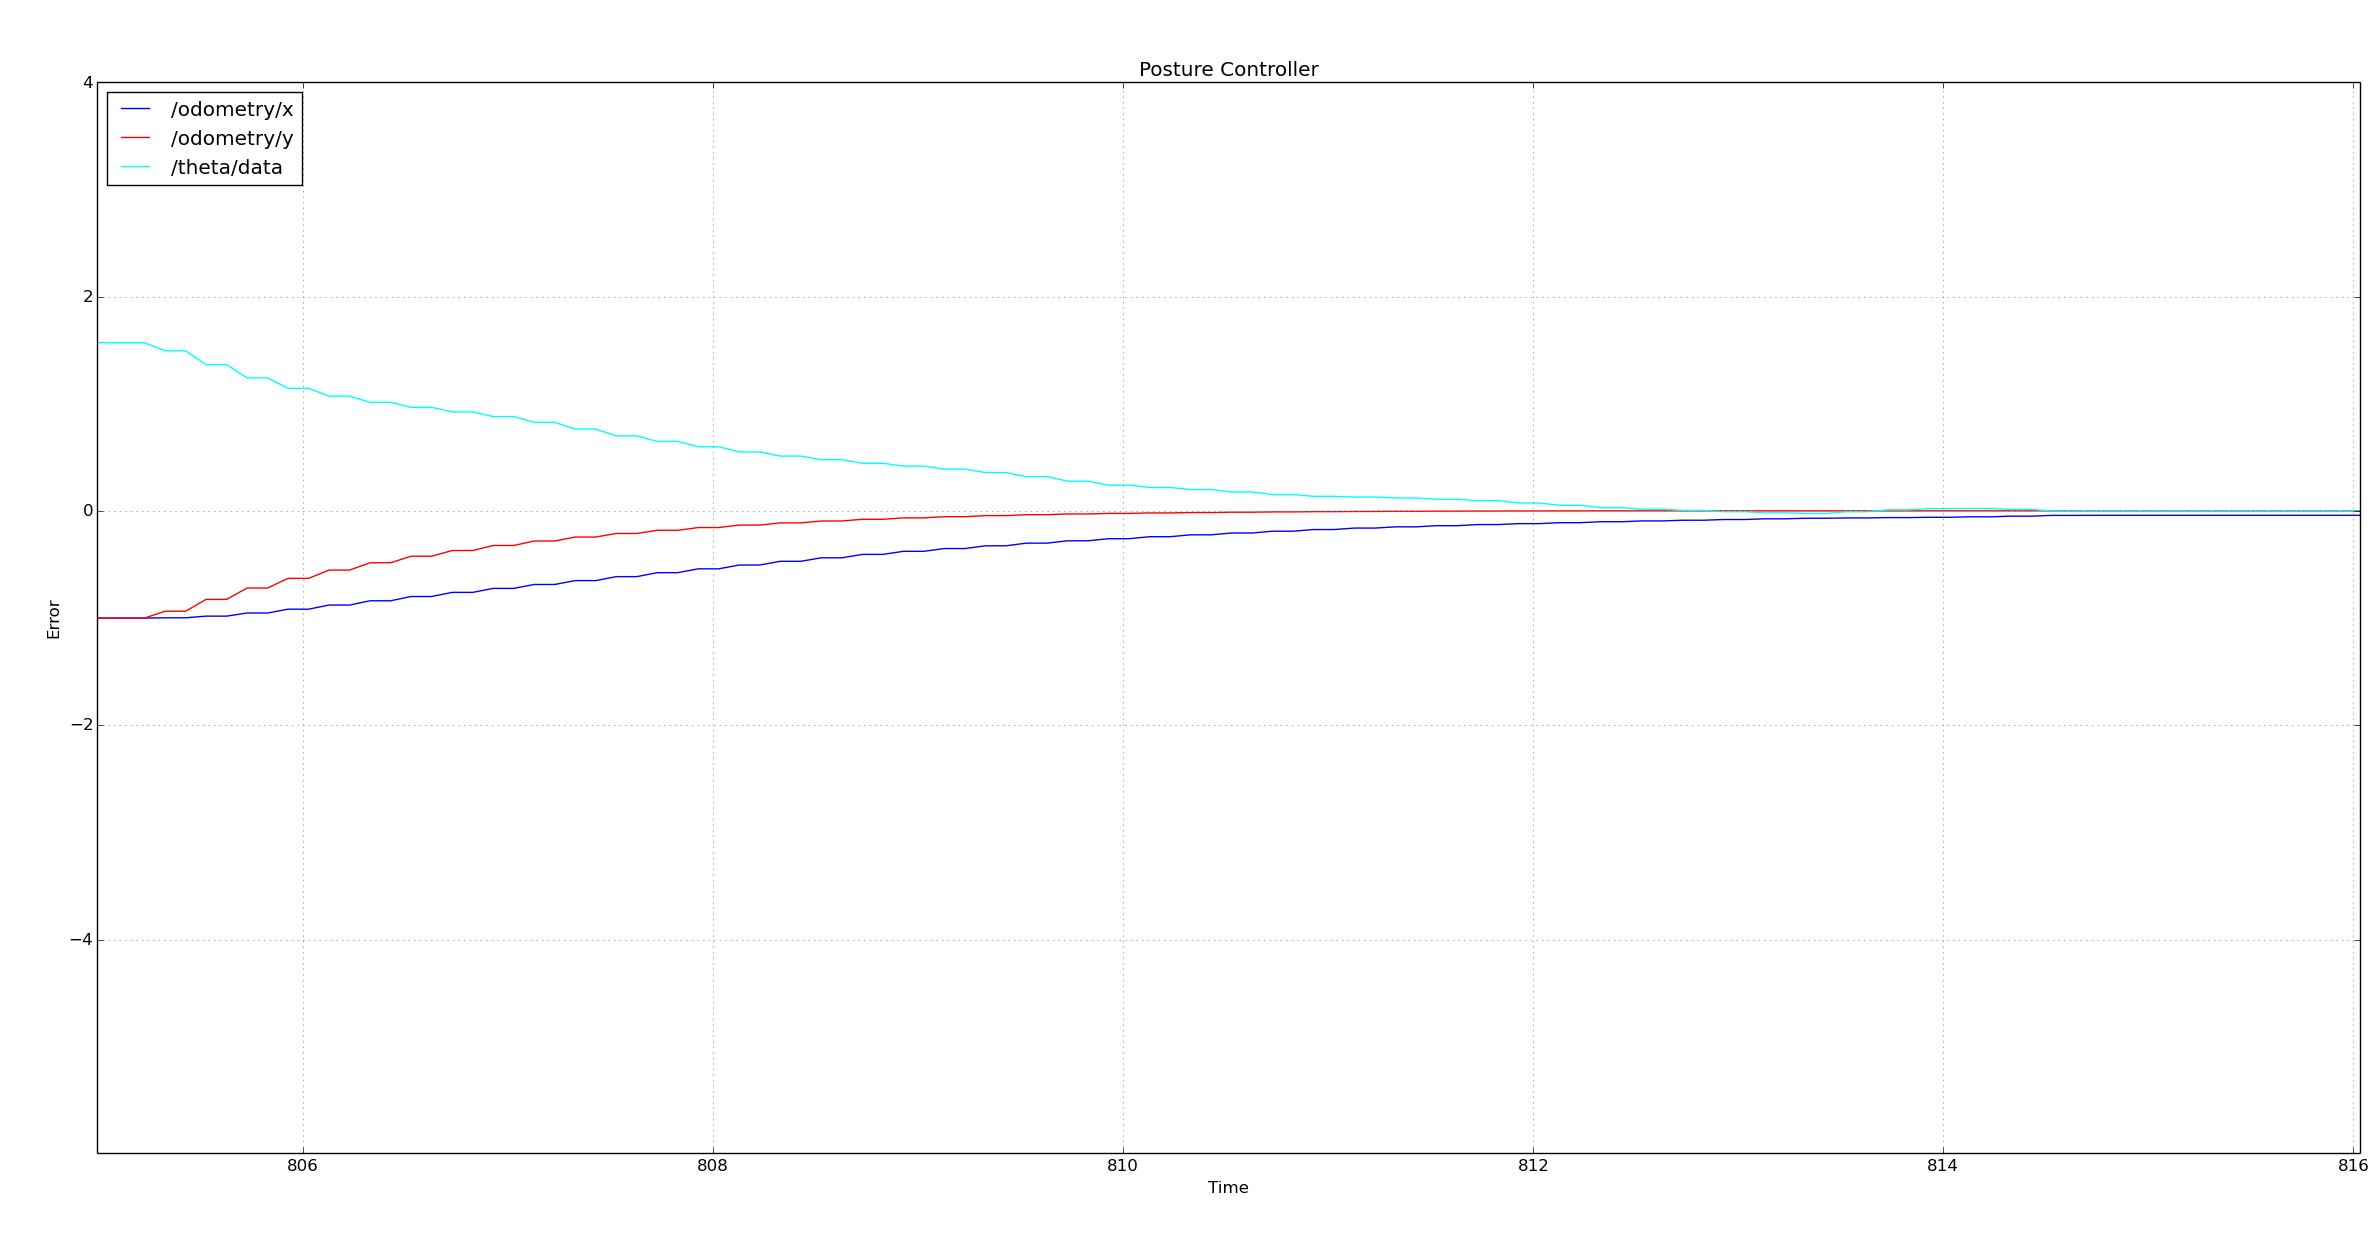
\includegraphics[width=0.9\textwidth]{rover2_rqt_plot94_2413.png}
		%\caption{code}	
 		%\label{fig:3}
		\end{figure}				 
	
		We tried different regulator parameters;

		\begin{figure}[H]
		\centering
		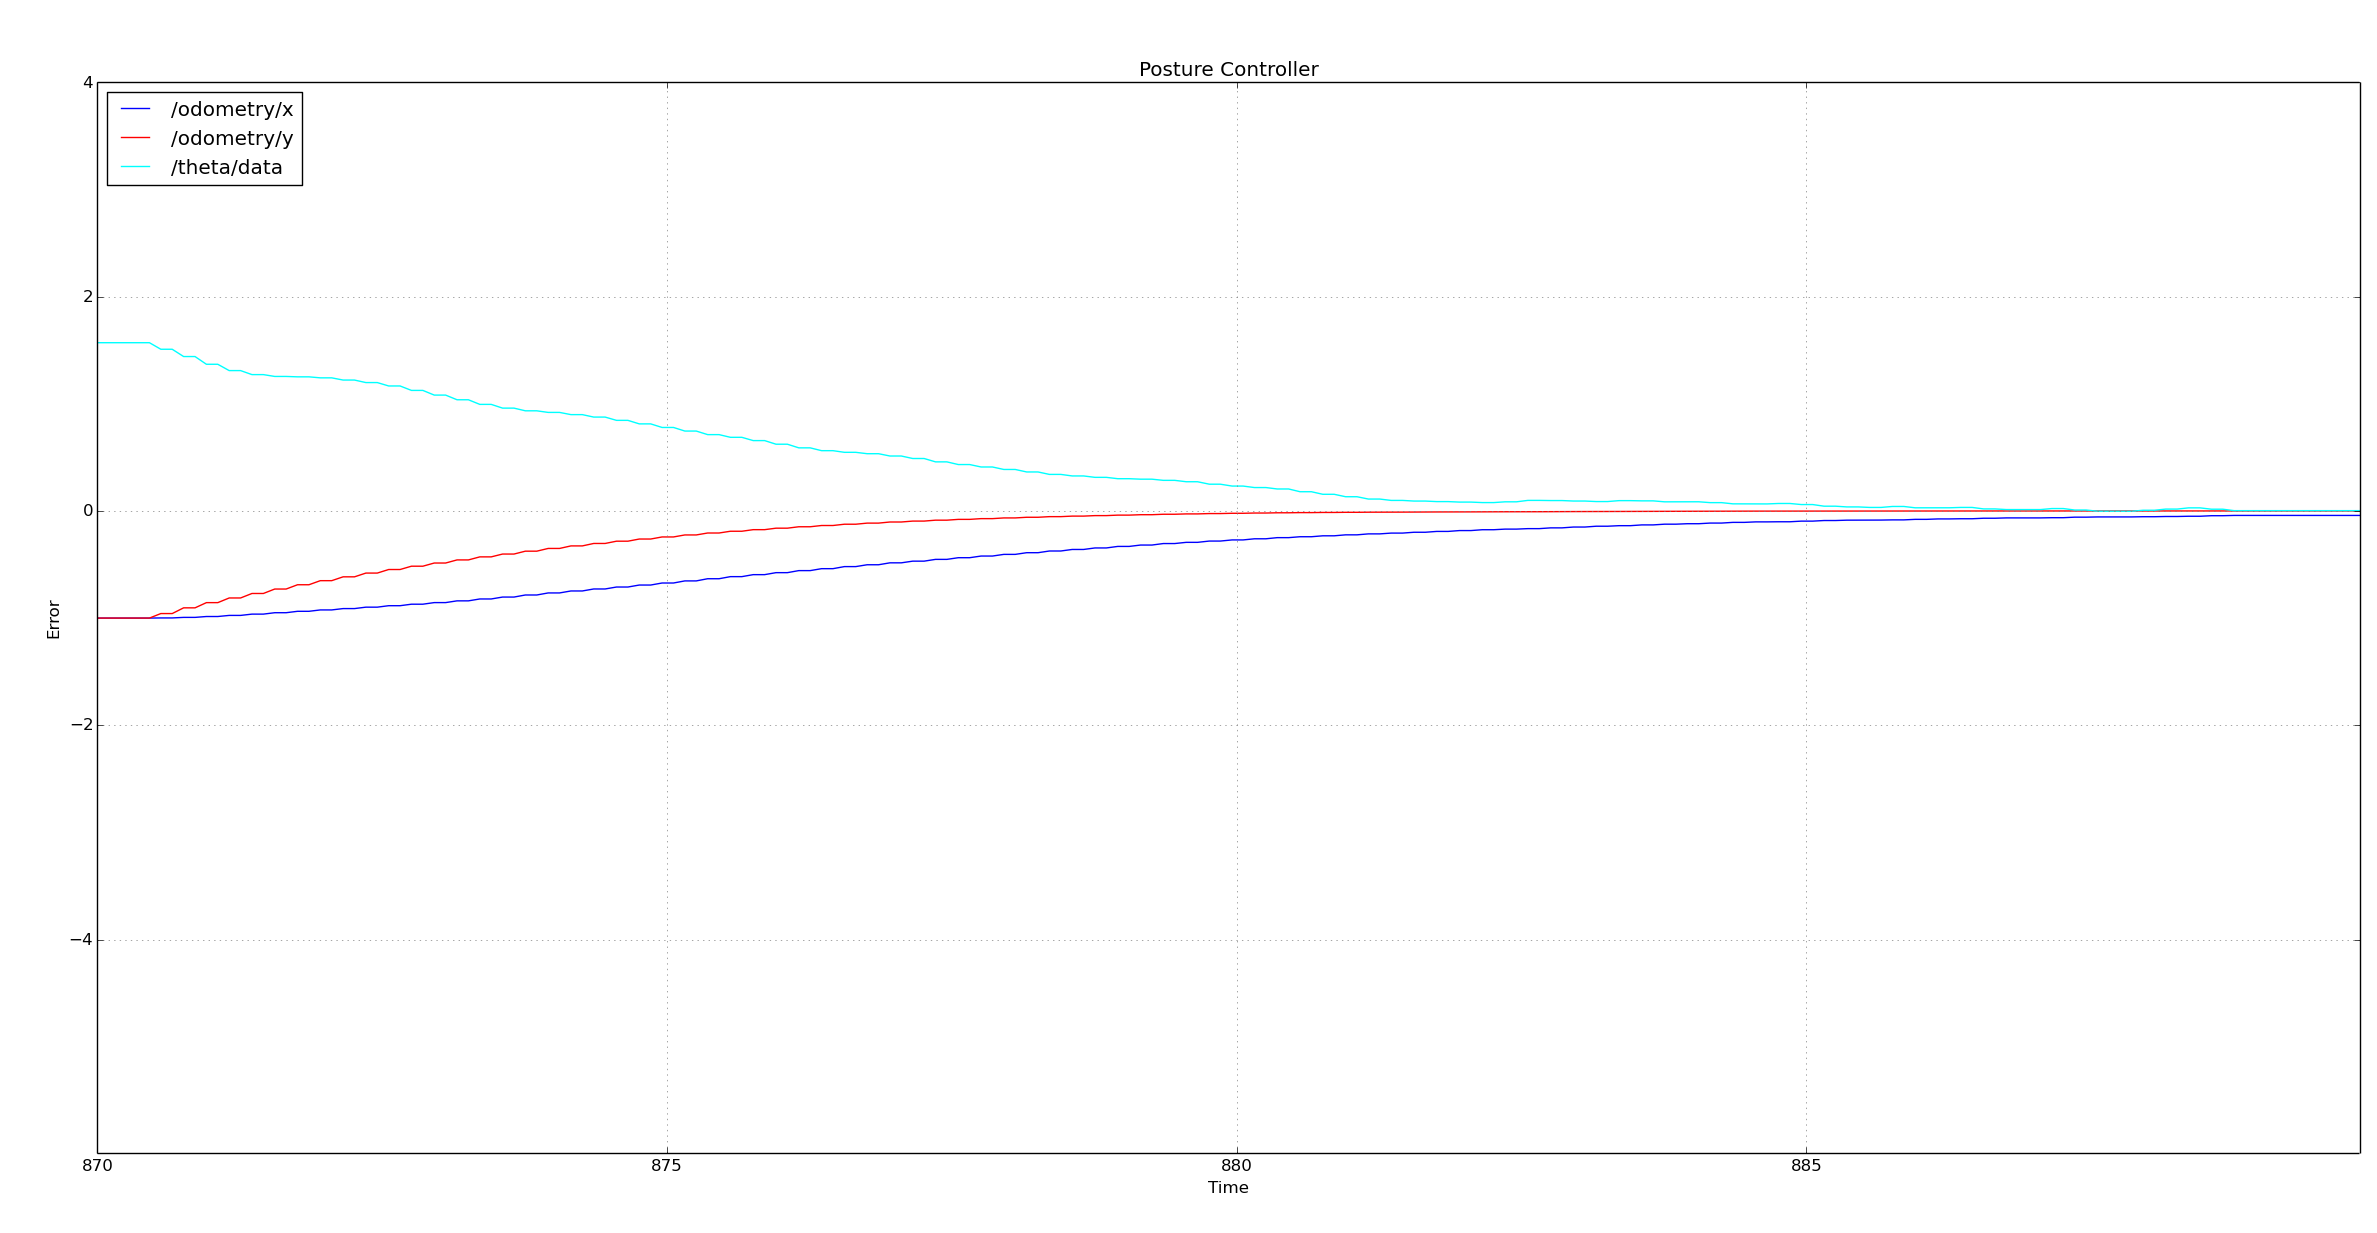
\includegraphics[width=0.9\textwidth]{rover2_rqt_plot94_167.png}
		%\caption{code}	
 		%\label{fig:3}
		\end{figure}


		The 1 6 7 regulator was also very accurate, ecpecially at distances < 2m. The 2 4 1.3 regulator was very accurate at all distances and was also very fast, so we turned up going for this regulator.





		The 2 4 1.3 regulator preformed like this;

		\begin{figure}[H]
		\centering
		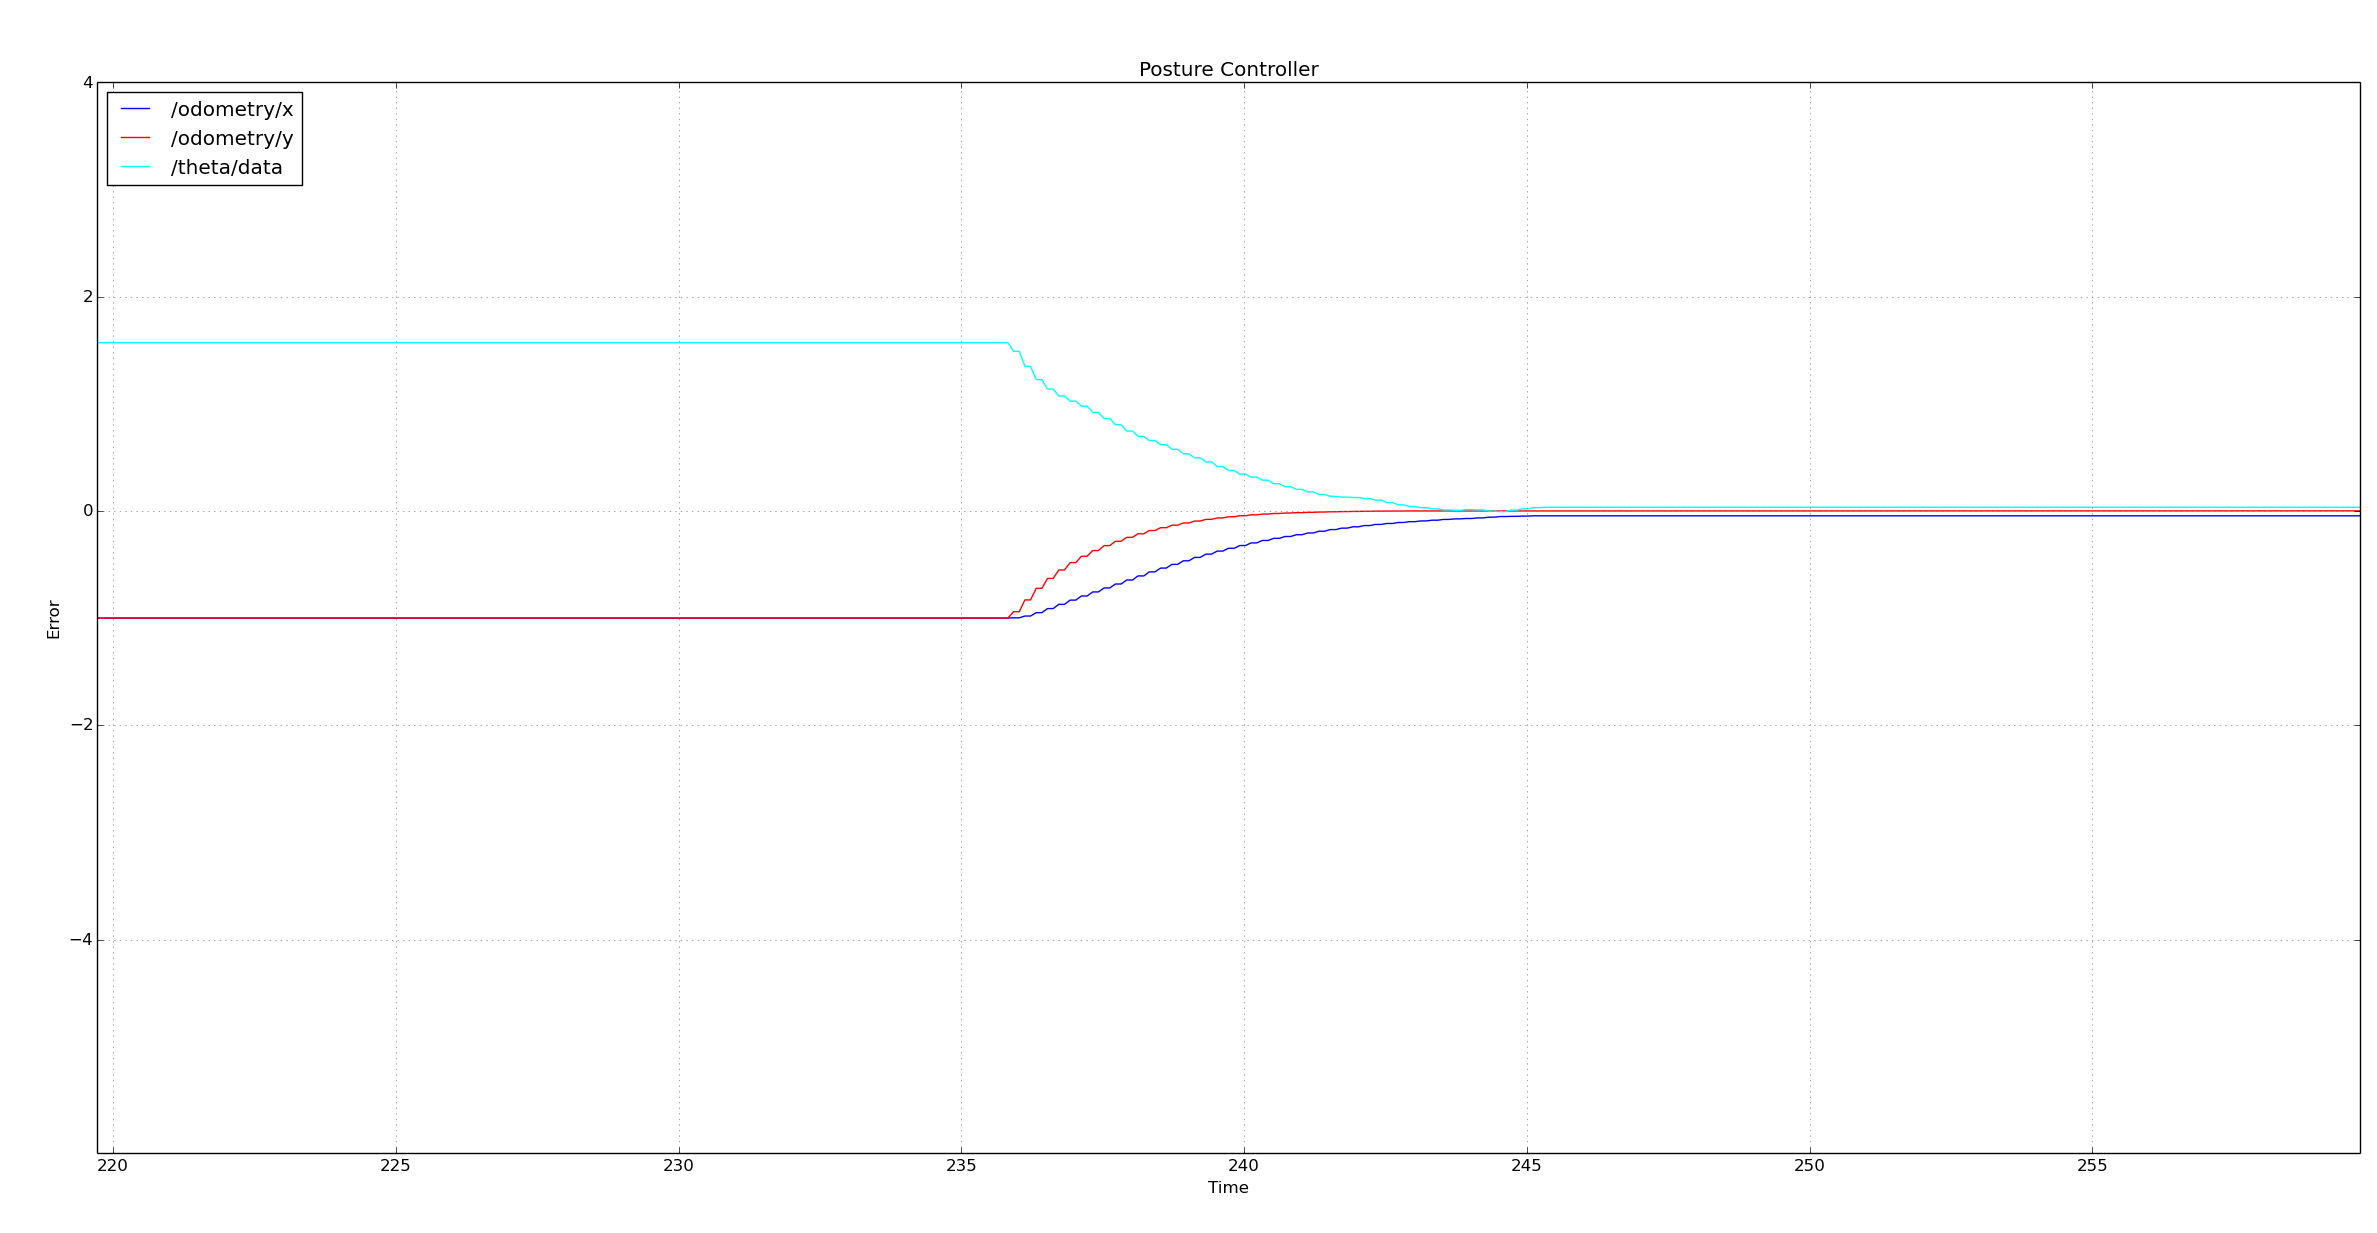
\includegraphics[width=0.9\textwidth]{rover2_rqt_plot9_0.png}
		%\caption{code}	
 		%\label{fig:3}
		\end{figure}



		\begin{figure}[H]
		\centering
		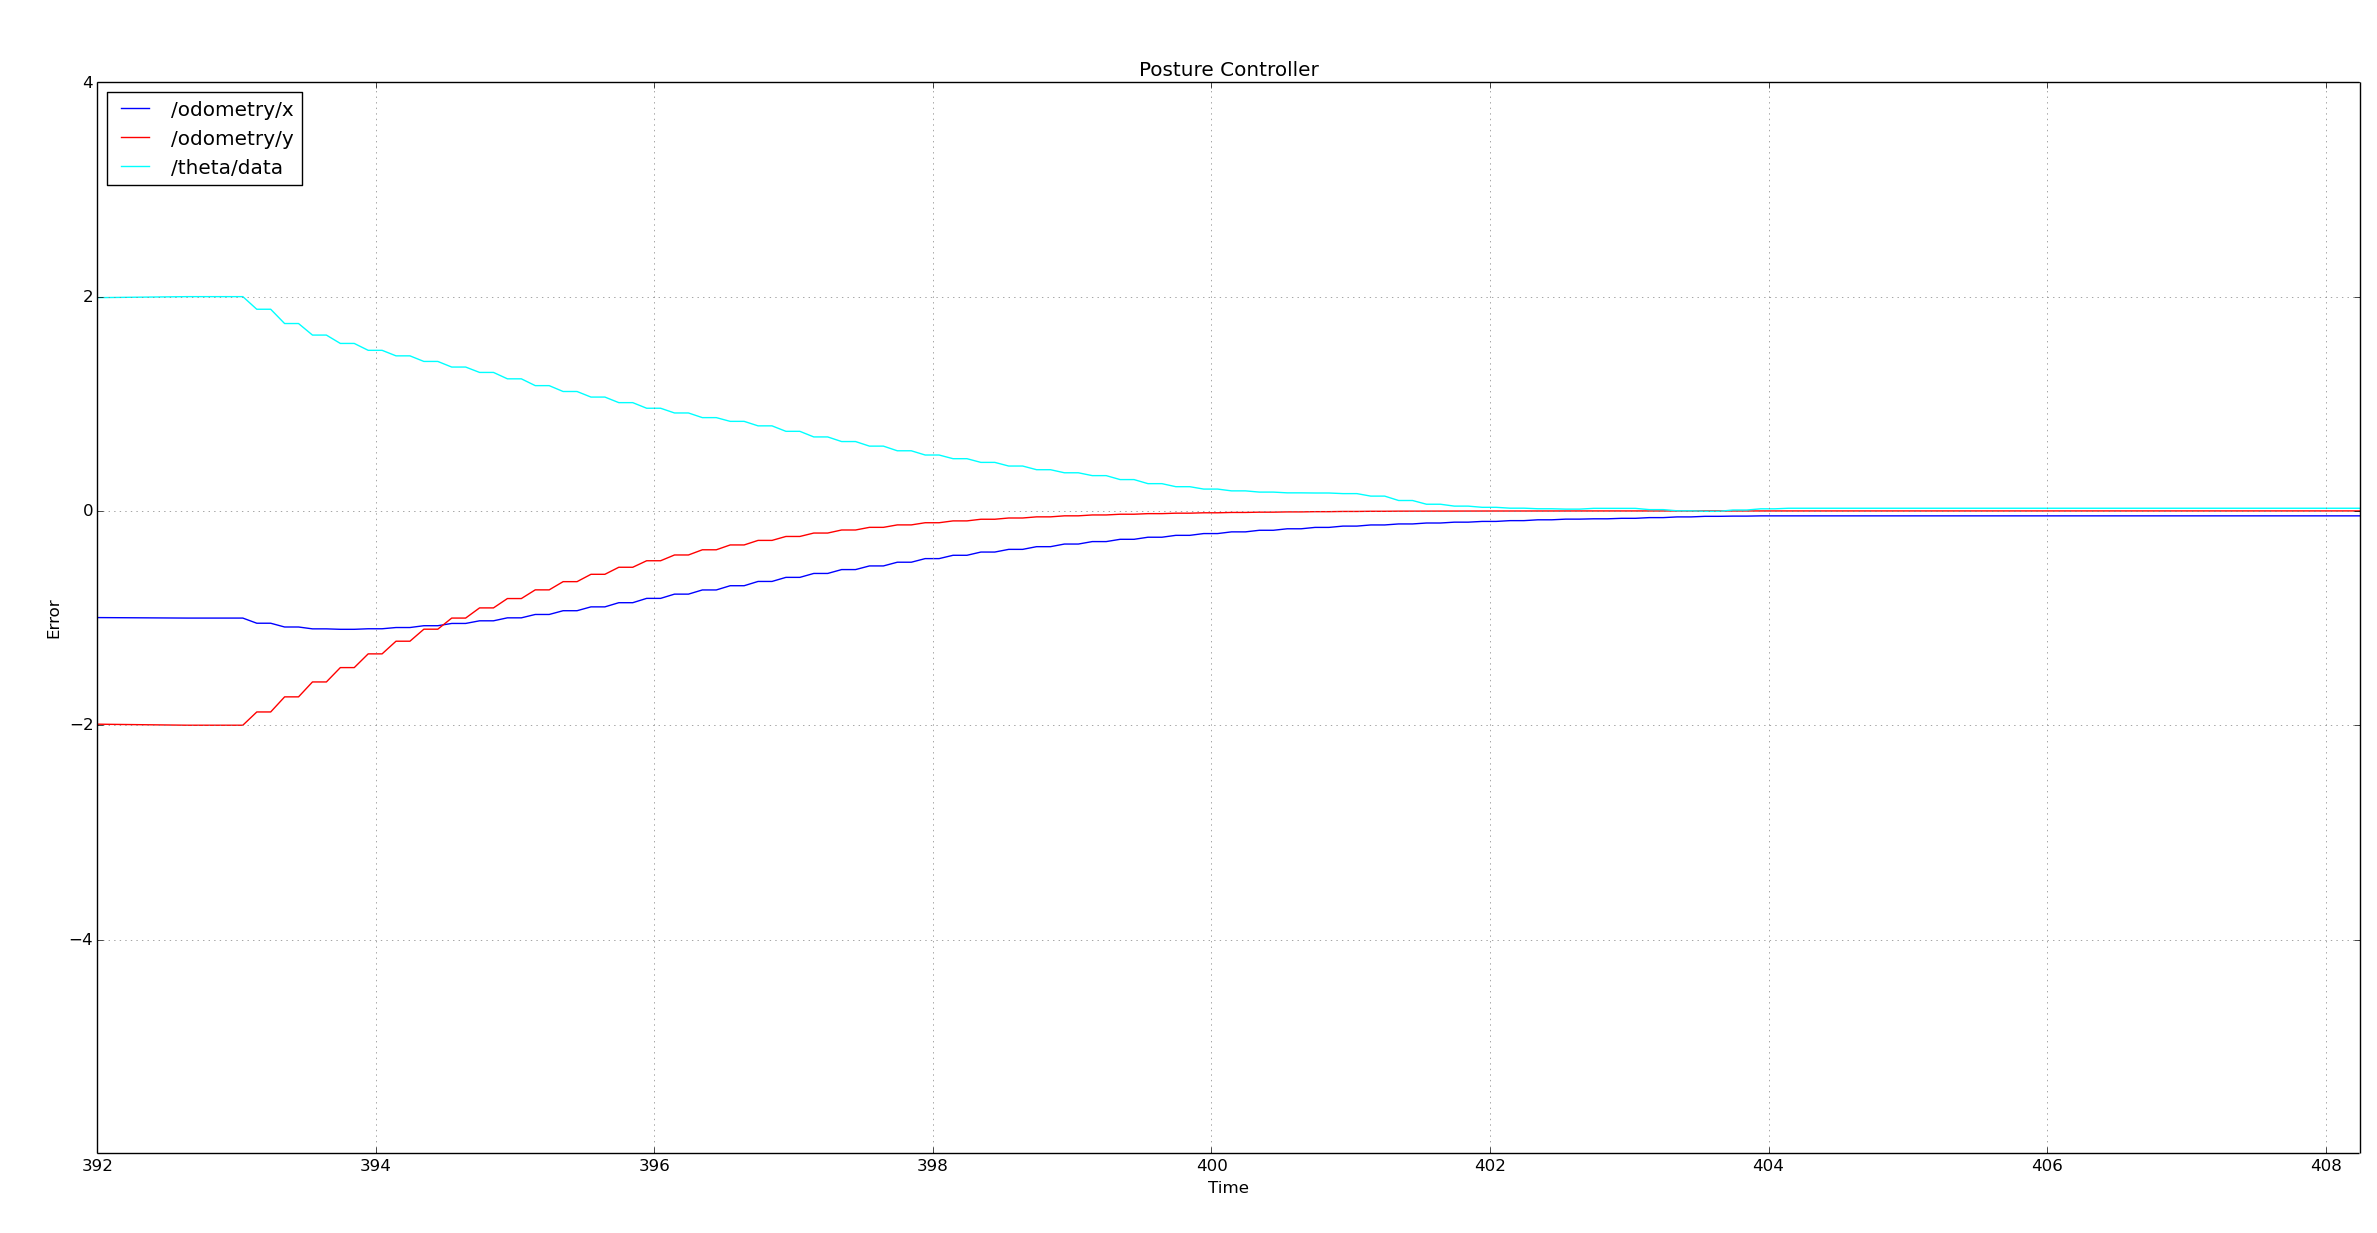
\includegraphics[width=0.9\textwidth]{rover2_rqt_plot91.png}
		%\caption{code}	
 		%\label{fig:3}
		\end{figure}



		\begin{figure}[H]
		\centering
		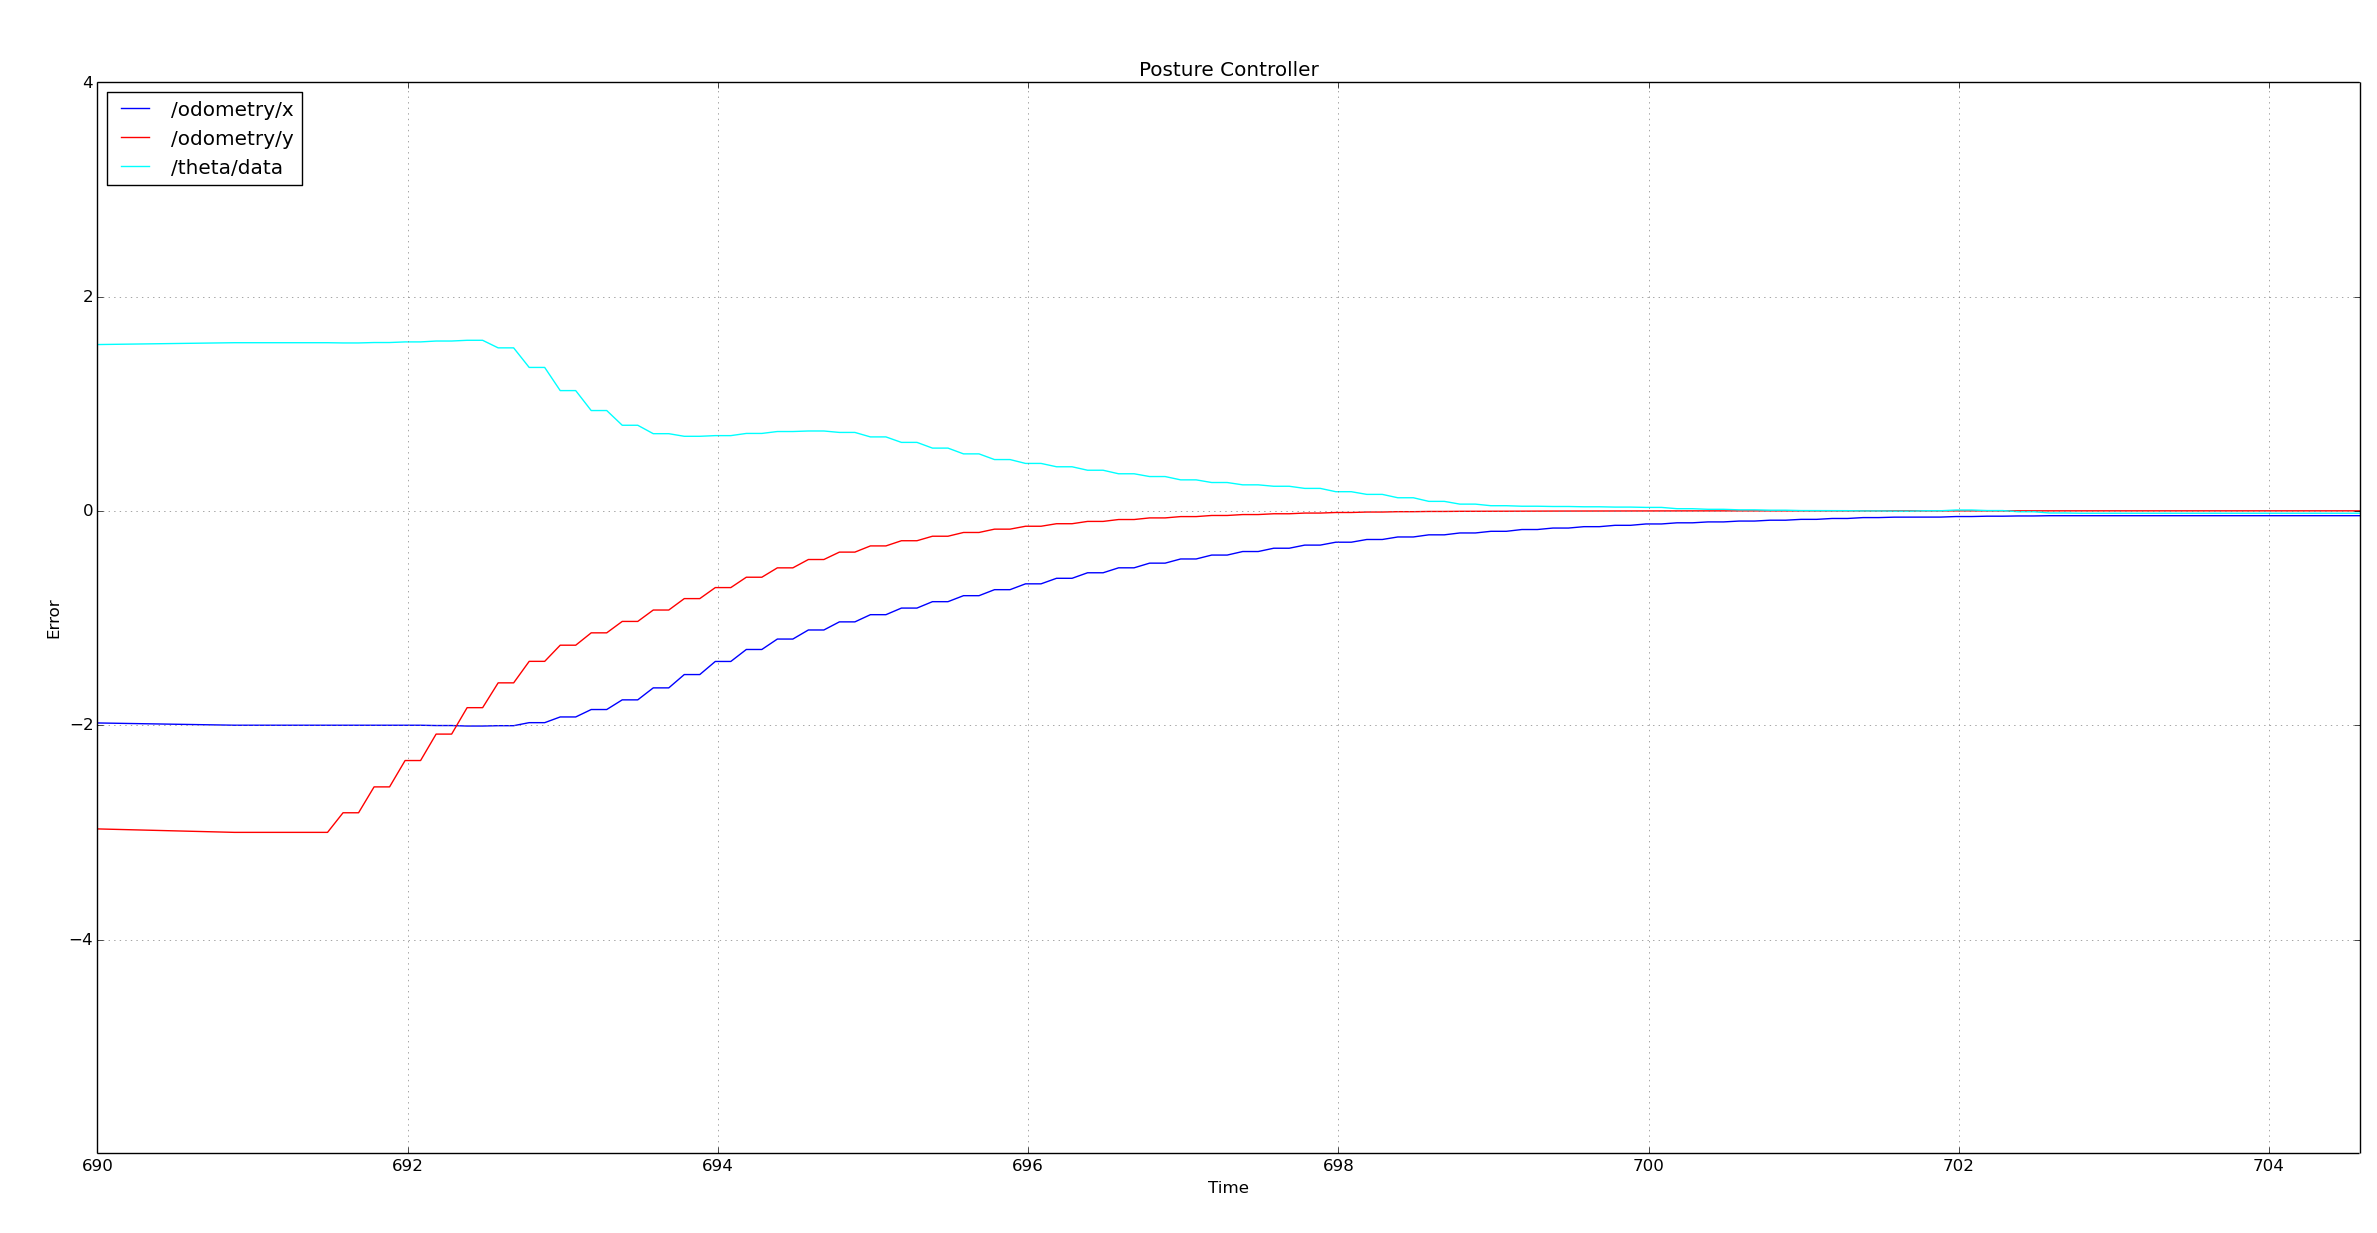
\includegraphics[width=0.9\textwidth]{rover2_rqt_plot93_high_error.png}
		%\caption{code}	
 		%\label{fig:3}
		\end{figure}


\end{document}
